\section{Hashgraph Consensus Mechanism} \label{sec:hashgraph_cm}
The Tagion network is based around a Hashgraph consensus algorithm and mathematical proof discovered by Leemon Baird \cite{SWIRLDS_HASHGRAPH}. This algorithm solves the Byzantine Generals’ Problem of generating a consensus order list of actions between distributed computer nodes connected in a network.
If more than 2/3 of the nodes follows the same consensus rules, all the nodes will, in finite time, reach the same order of events.
The network distributes the information via a gossip protocol, sending information about the data received from the other nodes in the network. All the nodes solving the Hashgraph algorithm will come to the same order of transactions.
Figure 1 below shows a Hashgraph of gossip information representing the information flow between network nodes. In finite time all nodes in the network will be able to build the same Hashgraph of gossip information.


\begin{figure}[ht]
 \centering
 % Replace this when we get the wavefront in
 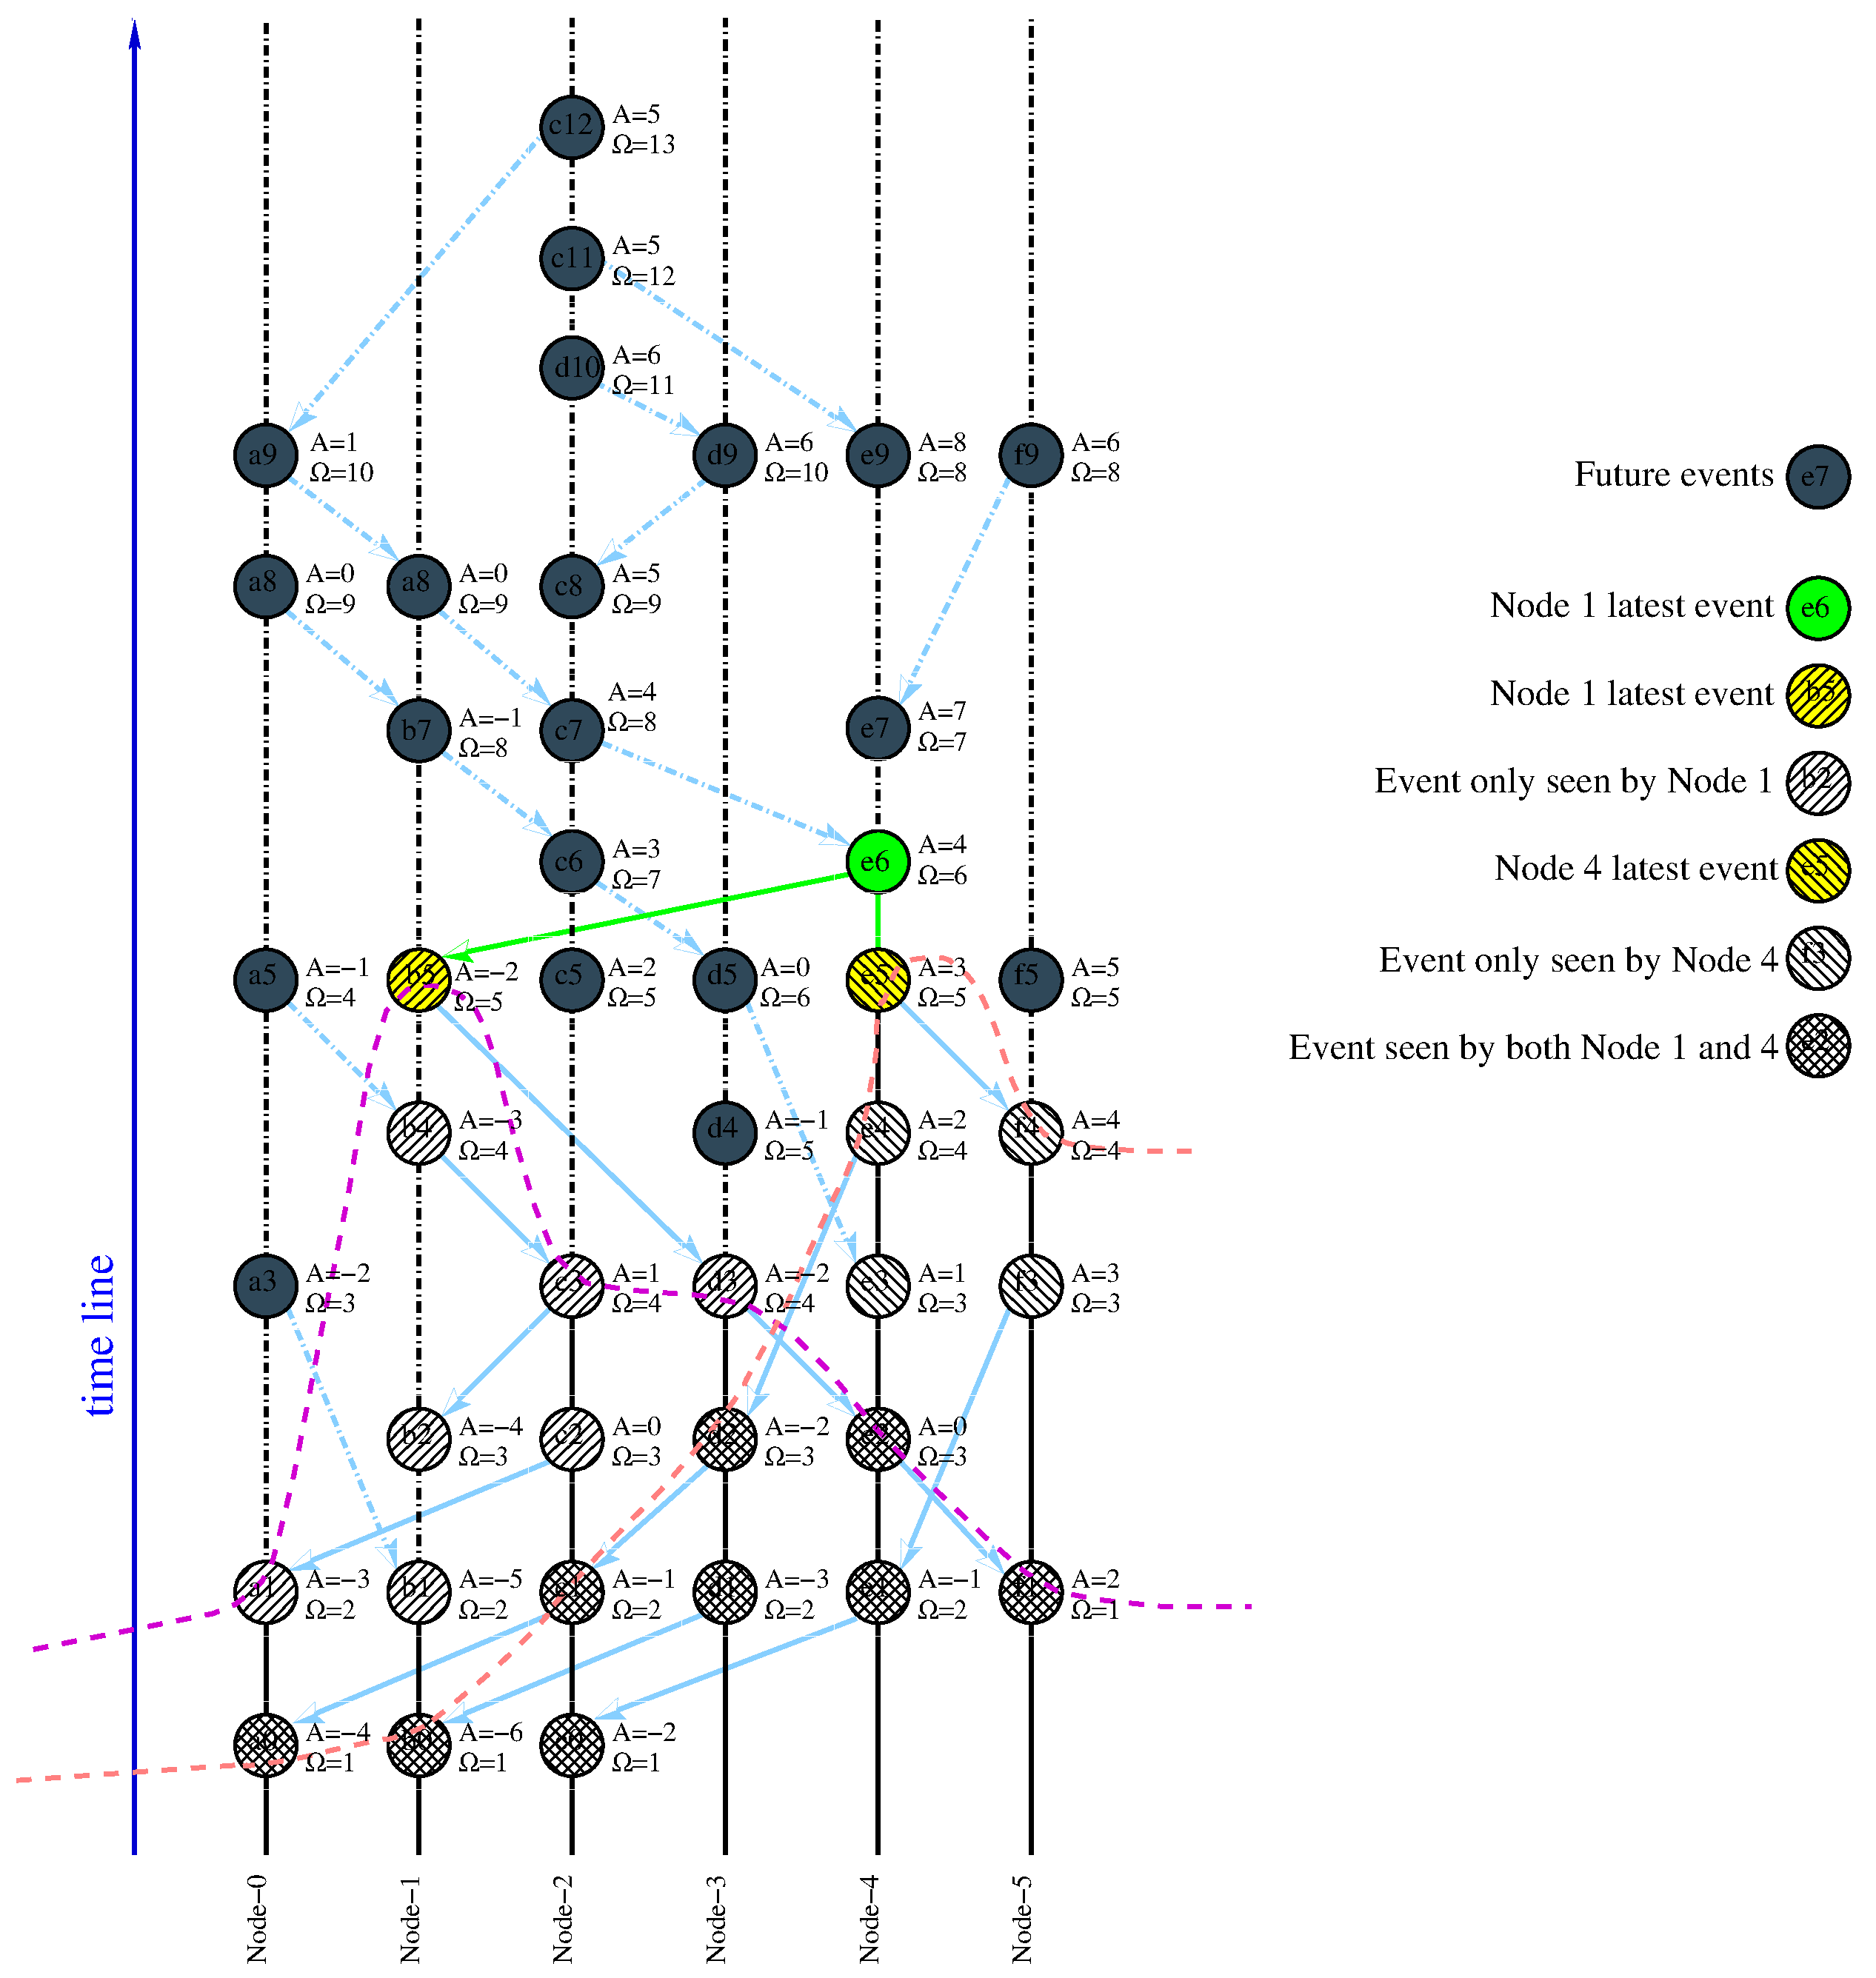
\includegraphics[width=0.7\textwidth]{fig/wavefront_and_order_long.eps}
% 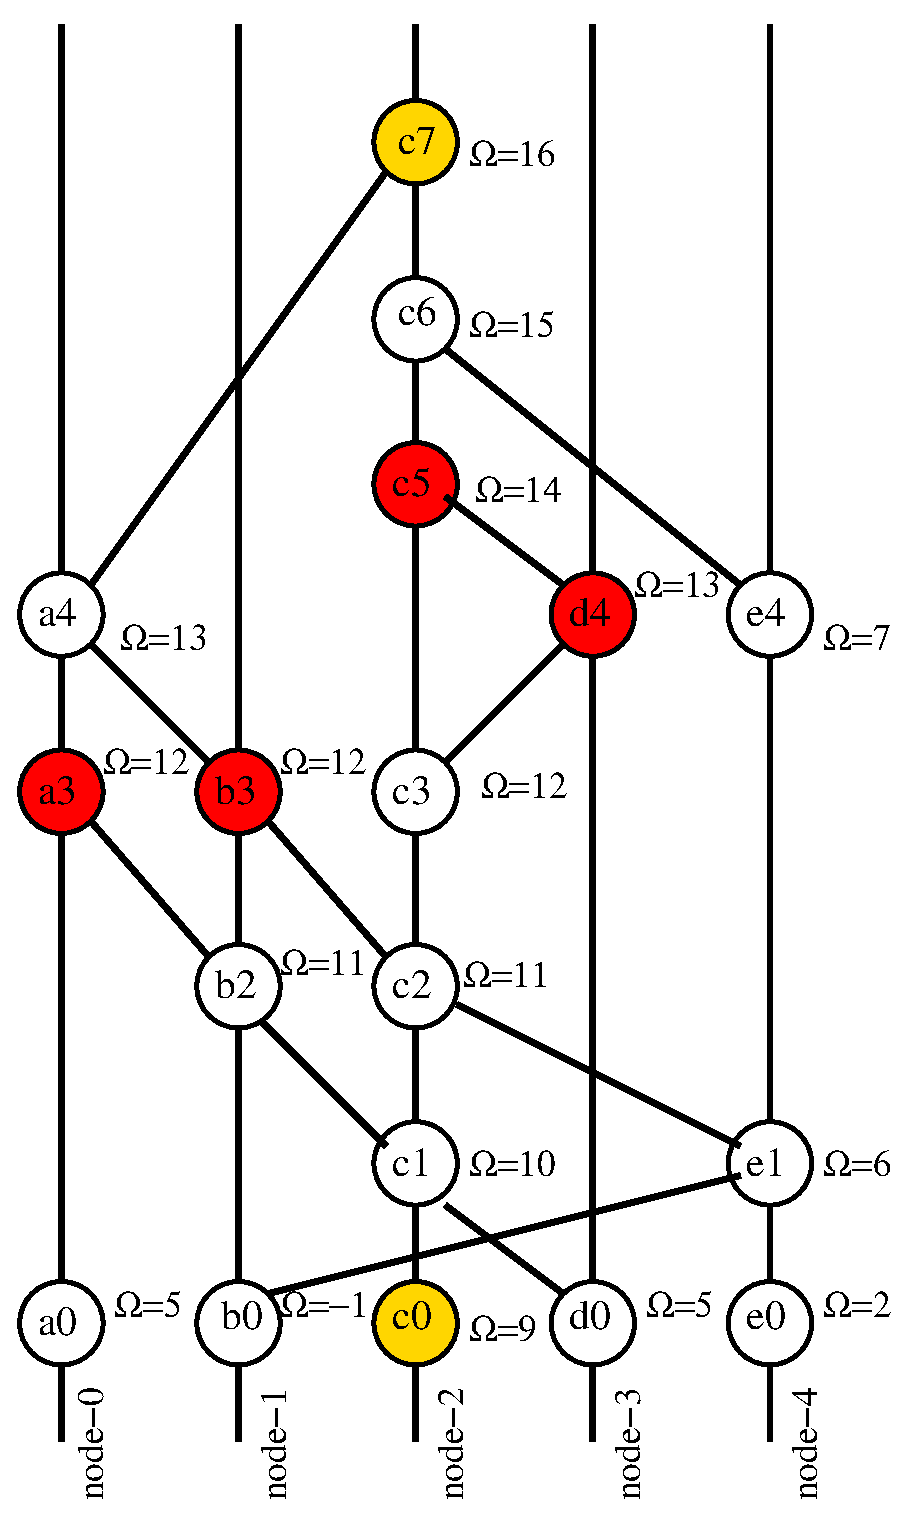
\includegraphics[width=0.45\textwidth]{fig/wavefront_and_order_small_no_alt.eps}
 % wavefront_and_order.eps: 3358x4625 px, 300dpi, 28.43x39.16 cm, bb=0 0 806 1110
 %\caption{Hashgraph with altitude(A) and parameter $\Omega$}
 \caption{Hashgraph with parameter $\Omega$}
 \label{fig:wavefront}
\end{figure}

% Hashgraph with altitude (A) order parameter Ω is shown. 
Each vertical line represents a compute node and each circle an event. The line between the events represents the communication of the events between the nodes. 
The events coloured red define a witness that is used to divide the consensus into rounds. Each round decides a list of events to be collected. This list of events is called an epoch and must be sorted into the same order as all other nodes. The description of the Hashgraph algorithm can be found in \cite{SWIRLDS_HASHGRAPH}.

% We take this out for now because of patent issues
\pagebreak

\subsection{Gossip protocol and Wavefront propagation}
The Hashgraph algorithm uses a gossip protocol called “gossip about gossip” to propagate information between the nodes. It means node A sends all the information of the communication that it knows to a randomly selected node B. This enables node B to construct the same Hashgraph as node A.

In the Tagion network, a protocol called Wavefront is used to exchange information between two nodes, ensuring that node A and B only need to communicate three times to share the state of the graph.
Each node keeps track of an integer value called Altitude. Altitude is increased by one for each event created by the node. Each node stores its current view of Altitude for each node in the network.
By exchanging information about the Altitude between two nodes, both can figure out if their Wavefront is higher and send a list of events which are in front.
The Wavefront information exchange has four states:

\begin{enumerate}
 \item 
 Node A selects random Node B and sends a list of all Altitudes. This state is called a tidal-wave.
 \item 
 Node B receives a tidal-wave from Node A. If Node B has already sent a tide-wave to Node A, then Node B will send what is called a breaking-wave to Node A. Otherwise Node B will return a list of all events which are in front of the tidal-wave of Node A. This state is called first-wave.
 \item 
 If Node A receives a first-wave from Node B, it returns a list of all the events which are in front of Node B. When this state has been reached the wavefront exchange ends.
 \item 
 If Node A or Node B receives a breaking-wave, the wavefront communication is dropped. This prevents both nodes from going into an infinity echo where they forever send information back and forth.
In the network, a node will often have many simultaneous wavefront connections so it will sometimes receive the same event package from other nodes. Then it will drop any duplicated events it receives.  
\end{enumerate}



\pagebreak

\subsection{Consensus Ordering}\label{sec:consensus_ordering}
In the Tagion implementation of the Hashgraph algorithm, an Event is only allowed to point to one or none ``other parent'' which is called a ``father-event'' as shown om \cref{fig:consensus_order}. This strategy aids in solving the graph forking problem and simplifies the consensus ordering.
The ``self-parent'' is defined as a ``mother-event'' in the Tagion implementation. An event must have a mother-event but doesn't have to have a father-event.

Each event points to the previous event called the mother-event, and some also point to another father-event. The mother-event is defined as the previous event from the same node. The father is an event sent via the gossip network from another node. 

The order $\Omega$ is calculated as:
\begin{equation}
 \Omega_{B,k+1} = max \big(\Omega_{A,k} , \Omega_{B,k} \big) +1
\end{equation}

The events in an epoch list are sorted by the order $\Omega$. According to \cref{equ:order} which define if an event A must be ordered before a B event. If the order of two events is equal, then the nested function $l'$ \cref{equ:nested_order} is use to decided the order.\\
A event is defined to be fatherless if the lineage of an event don't have a father back to the Eva event, and an Eva-event is defined to be an event without a mother and/or a father.
The following expression is used to order the events:

\begin{align}
 {l}(A,B) & = 
    \begin{cases}
         {l'}(A,B) &  	\text{if}  ~ ({\Omega}_{A} = {\Omega}_{B} )  \\ 
        {{\Omega}_{A} < {\Omega}_{B}} & 
        \text{otherwise}
    \end{cases} 
    \label{equ:order}    
\end{align}

\begin{align}
{l'}(A,B) & = 
\begin{cases}
{l}(A_{father},B_{father}) &  	
\text{if}  ~ (\text{A has a father} ~ \&  ~ \text{B has a father}) \\ 
{l}(A_{father},B_{mother}) &  	
\text{if}  ~ (\text{A has a father} ~ \&  ~ \text{B has a mother}) \\ 
{l}(A_{mother},B_{father}) &  	
\text{if}  ~ (\text{A has a mother} ~ \&  ~ \text{B has a father}) \\ 
{l}(A_{mother},B_{mother}) &  	
\text{if}  ~ (\text{A is not fatherless} ~ \&  ~ \text{B is not fatherless}) \\ 
0 &  	
\text{if}  ~ (\text{A is not fatherless}) \\ 
1 &  	
\text{if}  ~ (\text{B is not fatherless}) \\ 
{h}_{A} < {h}_{B} & 
\text{otherwise (Only happens for none orderd event)}
\end{cases} 
\label{equ:nested_order}    
\end{align}
If parameter $l(A,B)$ is $'true'$ if event A is ordered before event B (see \cref{sec:order_function}).

Note. An event which are fatherless is not allowed to contain a payload and an node must have participated in producing one epoch before the payload can be considered valid. 

\begin{figure}[H]
 \centering
 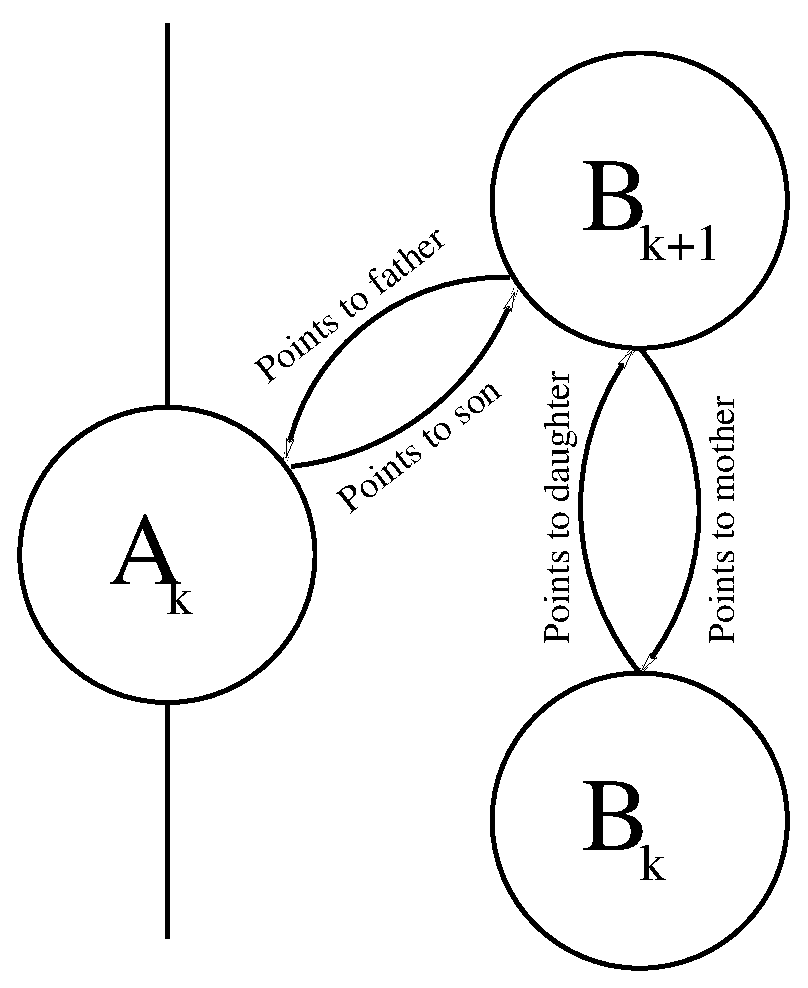
\includegraphics[width=0.5\textwidth]{fig/consensus_order.eps}
 % consensus_order.eps: 1550x1908 px, 300dpi, 13.12x16.15 cm, bb=0 0 372 458
 \caption{Events and relations}
 \label{fig:consensus_order}
\end{figure}

